\documentclass{bakalarka}
%\usepackage[cp1250]{inputenc}
\usepackage{listings}
\usepackage[utf8]{inputenc} 
\usepackage[czech]{babel}
\usepackage{ae}
\usepackage{fancyhdr}
\usepackage{float}
\usepackage{graphicx}
\usepackage{multirow}
\usepackage{color, colortbl}
\usepackage{enumitem}
\usepackage{array}
%\usepackage[pdftex]{graphicx}

\lstset{language=Java,keywordstyle=\color{blue}, commentstyle=\color{Green},stringstyle=\color{red},showstringspaces=false,breaklines=true,tabsize=3,basicstyle=\footnotesize}



\author{Martin Kadlec}
\title{Docházka a výkazy práce pro systém IMIS na platformě Android}
\titlet{}
\titlett{}
\university{Západočeská univerzita v Plzni}
\faculty{Fakulta aplikovaných věd}
\department{Katedra informatiky a výpočetní techniky}
\subject{Diplomová práce}
\town{Plzeň}
\begin{document}
\pagestyle{fancy}
\renewcommand{\chaptermark}[1]{\markboth{\textit{#1}}{}}
\renewcommand{\sectionmark}[1]{\markright{\textit{#1}}{}}
\cfoot{\thepage}
\lhead{\leftmark}
\rhead{\rightmark}
\maketitle
\chapter*{Prohlášení}
\thispagestyle{empty}
Prohlašuji, že jsem bakalářskou práci vypracoval samostatně a výhradně s~použitím citovaných pramenů.
\vskip 1.5em
V Plzni dne \today
\vskip 0.7em
\hskip 9cm Maxipes Fík
\chapter*{Abstract}
\thispagestyle{empty}
Text of abstract.
\pagestyle{empty}
\tableofcontents
\pagestyle{fancy}
\renewcommand{\chaptermark}[1]{\markboth{\textit{#1}}{}}
\renewcommand{\sectionmark}[1]{\markright{\textit{#1}}{}}
\cfoot{\thepage}
\lhead{\leftmark}
\rhead{\rightmark}
\parskip 1em

%\renewcommand{\chaptermark}[1]{\markboth{\textit{#1}}{}}
%\renewcommand{\sectionmark}[1]{\markright{\textit{#1}}{}}
\chapter{Úvod}

\chapter{Současný systém}
IMIS = Integrovaný manažerský informační systém

\section{Oracle forms}
Oracle forms je softwarový produkt vyvinutý společností Oracle. Slouží k vytváření formulářů, které interagují s Oracle databází. Jako programovací jazyk využívá PL/SQL. Produkt byl původně požíval terminálové rozhraní pro komuikaci se serverem. Později byl přepracován do architekrury klient-server.\\ \indent
Prostředí běhu zajišťuje defaultní správu transakcí. Díky tomu je Oracle Forms silný nástroj pro efektivní vývoj aplikací, jejichž primárním cílem je přístup k datům uložených v databázi. 

\paragraph{PL/SQL}
PL/SQL (Procedural Language/Structured Query Language) je procedurální nadstavba jazyka SQL od firmy Oracle založená na programovacím jazyku Ada.

\section{Architektura}

\begin{figure}[H]
  \centering
  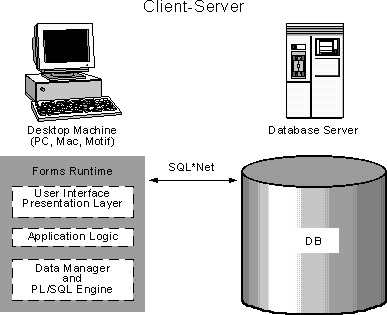
\includegraphics[scale=0.8]{obr/d2k_wea2.png}
  \label{}
\end{figure}
TODO asi vyrobit vlastni

\section{Komponenty formuláře}
Z hlediska architektury se Oracle Forms aplikace skládá z těchto celků:

\subsection{Moduly}

\paragraph{Modul formuláře} 
Modul formuláře je hlavní komponenta aplikace. Poskytuje kód nezbytný pro interakci s úložištěm a uživatelským rozhraním. 
Data poskytovaná databází jsou reflektovaná v prvcích uživatelského rozhraní jako jsou textová pole, zaškrtávací políčka, přepínače, talčítka atd. Formulář je logicky organizován do bloků. Existují dva typy bloků: 
\begin{itemize}
\item Datový blok\\ Datový blok zobrazuje zdrojová data a poskytuje abstrakci pro způsob jakým jsou tato data získávána. Blok může být asociován s databázovou tabulkou, databázovým pohledem, uloženou procedurou, dotazem do databáze nebo transakčním triggerem. Asociace datového bloku a databázových dat standartně umožnujě přístup k těmto datům a jejich modifikaci.\indent
Datové bloky mohou být navzájem svázany vztahem "rodič - potomek". Takový vztah představuje relaci 1:N databázových tabulek. Oracle Forms zajišťuje to, že při spojení mezi master a detail bloky se zobrazí pouze ty detail bloky, které jsou vázány na master blok přes cizí klíč. 

\item Řídící blok \\
Představuje blok, který nemá vztah k databázové tabulce. Řídící blok může obsahovat jakékoli prvky uživatelského rozhraní. Prvky mohou sloužit k uložení dočasných proměných nebo k zobrazení dat, které nemají přímou vazbu s databází. 
\end{itemize}

\paragraph{Modul menu} 
Modul obsahuje hiearchii menu. Každé menu obsahuje zvolitelné položky. Každý formulář obsahuje defaultní menu obsahující příkazy pro základní DML operace s databází CRUD.

\paragraph{Modul PL/SQL knihovny}
Modul obsahuje znovu využitelný kód, který může být využit jinými formuláři, menu či knihovnami. Programové jednotky knihovny mohou být fuknce, procedury a balíčky. Programové jednotky jsou spouštěny na straně klienta. Mohou obsahovat business logiku. Knihovny jsou nezávislé na formuláři, jsou zaváděny dynamicky a mohou být zároveň využívány více formuláři.

\paragraph{Modul knihovny objektů}
Modul obsahuje znovu využitelné objekty. Řeší uskladnění, správu a distribuci těchto objektů, které mohou být využity jinými formuláři, menu či knihovnami. Využívání tohoto modulu přináší přínosy v podobě úspory paměti při běhu aplikace.

\begin{figure}[H]
  \centering
  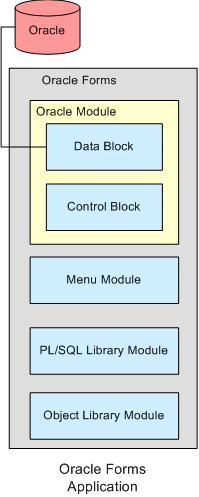
\includegraphics[scale=0.8]{obr/forms_arch3.png}
  \label{}
\end{figure}
TODO obrazek upravit - prepsat Oracle Module na Form Module

\subsection{Triggery}
Aplikace v Oracle pracuje s následujícími typy triggerů:
\begin{itemize}
\item Block-processing triggers - jsou spouštěny při události na položce patřící tomuto bloku.
\item Interface event triggers - jsou spouštěny při události v uživatelském rozhraní formuláře.
\item Master-detail triggers - jsou spouštěny při události související se vztahem "rodič - potomek"  na daných blocích. Např. při změně položky rodiče příslušný trigger zobrazí správné položky v bloku potomka.
\item Message-handling triggers - zpracovávájí zobrazení chybových či informačních zpráv.
\item Navigational triggers - jsou spouštěny při navigaci po položkách formuláře.
\item Query-time triggers - jsou spouštěny na úrovni bloku před a po dotazu do databáze.
\item Validation triggers - jsou spouštěny při validaci záznamu v položce.
\item Transactional Triggers - vyvolají se při různých událostech související s interakcí s datovým úložištěm.
\end{itemize}
Pokud se jedná o datový blok, který je svázan s tabulkou v databázi, prostředí běhu automaticky zajištuje DML pro tyto bloky.
Pokud vývojář požaduje nestandartní akci při těchto úkonech, provede překrytí těchto triggerů s vlastní definovanou akcí.

\subsection{Seznam hodnot}
A (LOV) is a pop-up window that provides the user with a selection of values. The values can be static or populated by querying the database. LOVs are populated using columns returned by record groups. Check the Record Group property of the LOV for the record group which is used to provide values.

\section{Uživatelské rozhraní}
\begin{figure}[H]
  \centering
  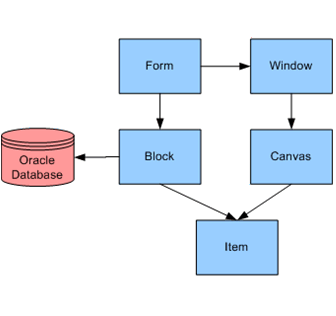
\includegraphics[scale=0.8]{obr/window.png}
  \label{}
\end{figure}
Plátno je objekt, na který je nakresleno celé GUI formuláře, tedy všechny viditelné objekty. Může mít prakticky jakoukoli velikost. Okno ohraničuje plochu plátna, která bude zobrazena. View řídí, jak bude plátno v určité době zobrazeno v okně.\\
TODO přepsat


\section{Datový model}

\section{Důležité formuláře}

\subsection{Zápis příchodů a odchodů}
\begin{figure}[H]
  \centering
  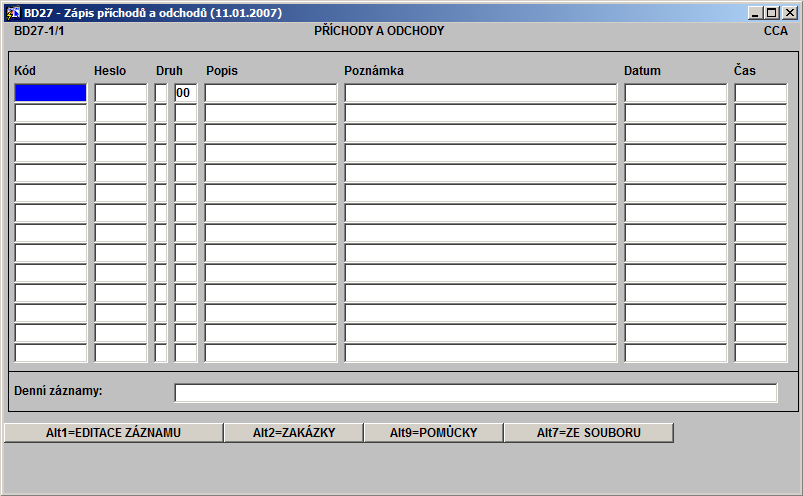
\includegraphics[scale=0.6]{obr/BD27.png}
  \label{}
\end{figure}
+popsat z pohledu uzivatele
\subsection{Výkaz práce}
\begin{figure}[H]
  \centering
  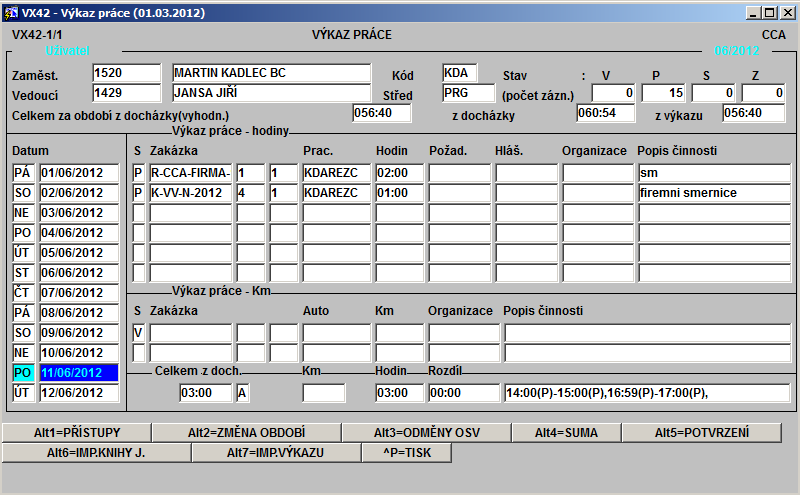
\includegraphics[scale=0.6]{obr/VX42.png}
  \label{}
\end{figure}
+popsat z pohledu uzivatele

\chapter{Analýza}

\section{Architektura}
Při návrhu architektury jsem se rozhodoval mezi třemi variantami: přímé spojení Android aplikace ke vzdálené databázi pomocí JDBC, synchronizaci dat se vzdálenou databází pomocí Oracle Database Mobile Server a nakonec využití webové služby, která by sloužila jako rozhraní mezi klientskou aplikací a databázovým serverem.

\subsection{Přímé připojení k databázi}
Přestože příme připojení k Oracle databázi pomocí JDBC je možné, tuto variantu jsem zamítl. Připojení pomocí JDBC je primárně určeno pro stabilní síťové připojení, které má malou odezvu a nízkou ztrátu paketů. Využití JDBC by přineslo problémy v podobě špatné odezvy aplikace, kvůli znovu navazování spojení a vytváření nových databázových relací, které musely být v důsledku ztráty konektivity ukončeny.\\ \indent
Vzhledem k tomu, že původní Forms aplikace funguje jako tlustý klient, provádí veškerou bussines logiku. Tato logika je zapotřebí ke správné funkčnosti systému. Bylo by tedy nutné přenést tuto logiku na stranu klienta a potřeba komunikace se vzdálenou databází by byla větší než k pouhému přenesení dat.

\subsection{Oracle Database Mobile Server}
Oracle Database Mobile Server 11g je server zajišťující  synchronizaci dat mezi Oracle databází a mobilními zařízeními. Klíčovou vlastností tohoto produktu je synchronizační jádro, které je schopné zajistit synchronizaci velké počtu mobilních zařízení se vzdálenou databázovým systémem. Přestože bylo toto synchronizační jádro navrženo pro stabilní připojení, je schopné zajistit spolehlivou funkci i při nestabilním připojení. V případě, že je spojení přerušeno synchronizace je pozastavena a po navázání spojení pokračuje v místě přerušení. Dále umožuje šifrování dat, jak pro přenos tak i pro jejich persistenci.\\ \indent
Tato varianta byla zamítnuta protože řeší pouze synchronizaci dat a neumožňuje zajistit provedení business logiky. Dalším důvodem je skutečnost, že její použití by vyžadovalo zakoupení licence pro tento server.\\ \indent
Server je možné spustit na serverech Oracle WebLogic Server a Oracle Glassfish. Mobilní klient, který běží na straně mobilního zařízení zajišťuje správu zařízení nutnou k synchronizaci. Tento klient je dostupný pro platfromy Java, Android, Blackberry, Windows a Linux.
(http://www.oracle.com/technetwork/products/database-mobile-server/overview/index.html)

\subsection{Webová služba}
Jako použitou architekturu jsem zvolil použití webové služby, která bude fungovat jako rozhraní mezi klientskou aplikací a databázovým serverem. Android klient v této architektuře funguje jako tenký klient spravující jen část funkčnosti z původního tlustého klienta. Business logika je umístěna na straně webové služby. Díky tomu že, webová služba bude umístěna v blízkosti firemní databáze, dojde k minimalizace odezev při zajištění business logiky systému. Mezi klientem a webovou službou se přenášejí pouzy data, která jsou opravdu nutná. \\ \indent
Z pohledu rozšiřitelnosti systému o další mobilní platformy se toto řešení jeví rovněž výhodně. Business logika by nebyla implementována ani na klientských aplikacích jiných platforem. Při změne logiky bude potřeba úpravy v kódu pouze na straně webové služby. Cílová architektura na vyobrazena na obrázku \ref{obr:arch}

\begin{figure}[H]
  \centering
  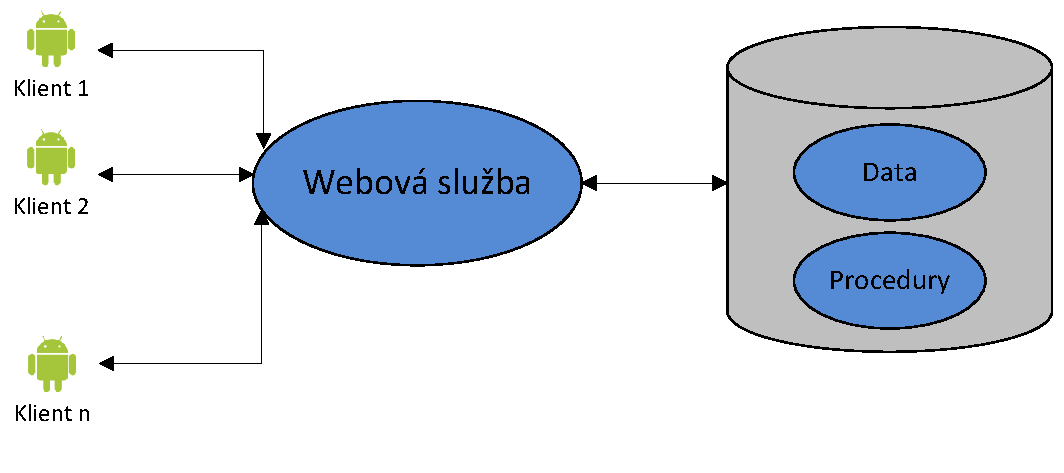
\includegraphics[scale=0.8]{obr/souc_arch2.pdf}
\caption{Zvolená architektura}
\label{obr:arch}
\end{figure}

\section{Výběr typu webové služby}

\subsection{Representational State Transfer}

\subsection{Simple Object Access Protocol}

\section{Datová vrstva}
\subsection{Práce s datumem a časem}
Při návrhu datového modelu jsem řešil problém pomocí jakého datového typu vyjadřovat údaj o čase či datu. V Oracle databázi je použit datový typ Date. SQLite databáze nabízí tři způsoby jako ukládat informaci o čase:
\begin{itemize}
\item \textbf{TEXT} podle ISO8601 normy ve formátu "YYYY-MM-DD HH:MM:SS.SSS".
\item \textbf{REAL} podle Juliánského kalendáře, počet dní od poledne 24. Listopadu roku 4714 před kristem (Greenwichského času).
\item \textbf{INTEGER} jako Unix Time, počet sekund 1970-01-01 00:00:00 UTC.
\end{itemize}

\noindent
Pro uložení v SQLite databázi jsem zvolil typ INTEGER. V aplikaci (Android klient, webová služba) jsem se rozhodl reprezentovat časový údaj pomocí primitivního typu long. Měl jsem k tomu řadu dobrých důvodů:
\begin{itemize}
\item odpadá starost s formátem datumu při serializaci a deserializace JSON řetězce
\item snadné porovnávání hodnot pomocí relačních operátorů
\item sníží se počet konverzí v aplikaci (např. pro výpočet pozice pro vykreslení komponenty v UI)
\end{itemize}

Také jsem se ujistil, že rozsah typu long je pro potřeby aplikace dostačující. Srovnání použitých datových typů je znázorněno v tabulce \ref{tab:cas}. 

\begin{table}[H]
\centering
\begin{tabular}{| c | c | c | c |}
\hline
Datový typ &  Minimální hodnota & Maximální hodnota & Přesnost \\ \hline
Oracle Date &   January 1, 4712 BCE  &  December 31, 4712 CE &  sekundy \\ \hline
SQLite INTEGER &    &  &  sekundy \\ \hline
Java long & 2.12.292269055 BC   & 17.8.292278994 AD &  milisekundy \\ \hline
\end{tabular}
\caption{Datové typy reprezentující časový údaj}
\label{tab:cas}
\end{table}

\subsection{Kritika datové vrstvy}
co se mi nelibilo a co bych navrhl jinak a jak, navrh prichody/odchody - jeden radek,
chybi primarni klic - ROWID jako unikatni identifikator, problemy ktere to prinasi,
format casu - problemy s prevodem

\section{Business logika}
existuje někajá možnost převodu formsů do javy - oracle adf - co to je, co to resi, proc to neresi muj problem
\subsection{Triggery}
jen ty, jejichž funkčnost bude muset být implementována.
\begin{itemize}
\item On-Delete, On-Insert, On-Update, Pre-Delete, Pre-Insert, Pre-Update
\item When-Validate-Item
\end{itemize}

\subsection{Databázové balíčky a uložené procedury}

\subsection{Forms knihovny}


\section{Uživatelské rozhraní}
\subsection{LOV}
jaka alternativa v androidu

\chapter{Zabezpečení}
Server webové služby je dostupná v síti VPN. LDAP + Spring security
\section{LDAP}
 Directory Access Protocol (LDAP) je internetový protokol definující přístup k distribuované adresářové službě. Podle tohoto protokolu jsou jednotlivé položky na serveru ukládány formou záznamů a uspořádány do stromové struktury. Protokol LDAP je byl navržen v souladu  se sadou standartů X.500 vyvinutých pro adresářové služby v počítačových sítích. Protokol LDAP je jejich odlehčenou verzí.\\ \indent
Aplikace funguje na bázi klient-server. Klient se při komunikaci se serverem autentizuje. Prostřednictvím klienta lze přidávat, modifikovat a mazat záznamy na serveru.

\subsection{Schéma}
Úkolem informačního modelu LDAP je definovat datové typy a informace, které lze v adresářovém serveru ukládat. Data jsou uchovávána ve stromové struktuře pomocí záznamů. Záznam představuje souhrn atributů (dvojice jméno - hodnota). Atributy nesou informaci o stavu daného záznamu. Záznamy, uložené v adresáři, musí odpovídat přípustnému schématu. Schéma  představuje soubor povolených objektových tříd a k nim náležících atributů.\\
Ukázka schématu definující strukturu záznamu zaměstnance:
\begin{verbatim}
objectclass ( 1.1.2.2.2 NAME 'zamestnanec'
                DESC 'zamestnanec firmy'
                SUP osoba
                MUST ( jmeno $ identifikacniCislo )
                MAY zkratkaZamestnance )
\end{verbatim}

Objekt popisující zaměstnance dědí od objektu osoba, vyžaduje povinný atribut 'jmeno' a 'identifikacniCislo' a nepovinny atribut 'zkratkaZamestnance'.

\subsection{Funkční model}
Funkční model umožňuje pomocí základních operací manipulovat a přistupovat k záznamům v adresáři a měnit či zjišťovat tak jejich stav.
\begin{itemize}[noitemsep,nolistsep]
\item Autentizační operace: Slouží k přihlášení a odhlášení uživatele pro komunikaci s adresářovým serverem. Jsou jimi míněny především operace bind a unbind. Na úspěšném provedení operace bind závisí výsledky aktualizačních a dotazovacích operací nad adresářem.
\item Aktualizační a dotazovací operace: Každý adresářový server podporuje základní operace s daty, jako je vyhledávání, přidávání, mazání, porovnávání a modifikace záznamů. Tyto operace bývají často spjaté s nastavením bezpečnostního modelu.
\end{itemize}

\subsection{LDAP URL}
Umístění zdroje je v LDAP specifikováno pomocí URL, které má následující tvar:
\begin{verbatim}
ldap://host:port/DN?attributes?scope?filter?extensions
\end{verbatim}
\begin{itemize}[noitemsep,nolistsep]
\item host - doména nebo IP adresa
\item port - síťový port (defaultně 389)
\item DN - význačné jméno použité jako základ pro vyhedávání
\item attributes -  seznam atributů
\item scope - specifikuje vyhledávácí rozsah  
\item filter - filtrovací kritérium
\item extensions - rozšíření
\end{itemize}

\chapter{Webová služba}

\section{REST}
Zdroj události

\definecolor{Gray}{gray}{0.9}
\renewcommand{\arraystretch}{1.5}
\begin{center}
\begin{tabular}{| m{2cm} |  m{10cm} |}
\hline
\rowcolor{Gray}
GET & events/\{icp\}?from=\{from\}\&to=\{to\} \\ \hline
&  \parbox{10cm}{Získá všechny události zaměstnance za dané období\\
Parametry:\begin{itemize}[noitemsep,nolistsep]
\item icp - identifikátor zaměstnance
\item from - datum začátku období
\item to - datum konce období
\end{itemize}} \\ \hline
\rowcolor{Gray}
DELETE  & events/\{rowid\} \\  \hline
&  \parbox{10cm}{Smaže danou událost\\
Parametry:\begin{itemize}[noitemsep,nolistsep]
\item rowid - identifikátor události
\end{itemize}} \\ \hline
\rowcolor{Gray}
POST  & events \\  \hline
&  \parbox{10cm}{Vytvoří událost, používá se bez parametrů protože identifikátor pro událost vytváří server
} \\ \hline
\rowcolor{Gray}
PUT  & events/\{rowid\} \\ 
&  \parbox{10cm}{Aktualizuje danou událost\\
Parametry:\begin{itemize}[noitemsep,nolistsep]
\item rowid - identifikátor události
\end{itemize}} \\ \hline
\end{tabular}
\end{center}

\noindent
Zdroj zaměstnanci
\begin{center}
\begin{tabular}{| m{2cm} |  m{10cm} |}
\hline
\rowcolor{Gray}
GET  & employees/\{icp\} \\ \hline
&  \parbox{10cm}{Získá seznam všech zaměstnanců, kteří jsou aktuálně v zaměstnaneckém poměru, obsahuje informaci zda jsou tito zaměstnanci podřízení, vzhledem k zaměstnanci identifikovém pomocí parametru\\
Parametry:\begin{itemize}[noitemsep,nolistsep]
\item icp - identifikátor zaměstnance
\end{itemize}} \\ \hline
\rowcolor{Gray}
GET  & employees \\ 
&  \parbox{10cm}{Získá poslední událost v docházce všech zaměstnanců, kteří jsou aktuálně v zaměstnaneckém poměru}\\
\hline
\end{tabular}
\end{center}

\noindent
Zdroj výkazy práce
\begin{center}
\begin{tabular}{| m{2cm} |  m{10cm} |}
\hline
\rowcolor{Gray}
GET  &records/\{kodpra\}?from=\{from\}\&to=\{to\} \\ 
&  \parbox{10cm}{Získá všechny výkazy práce zaměstnance za dané období\\
Parametry:\begin{itemize}[noitemsep,nolistsep]
\item kodpra - identifikátor zaměstnance (zkratka)
\item from - datum začátku období
\item to - datum konce období
\end{itemize}} \\ \hline
\end{tabular}
\end{center}
TODO uri authentikace?, test spojeni?

\chapter{Android aplikace}

\section{Funkcionalita}
Na základě analýzy současného systému a potřeb zaměstnanců byla vybrána k implementaci následující funkčnost: 
\paragraph{Docházka}
\begin{itemize}
\item Přehledné zobrazení událostí docházky daného zaměstnance
\item Uživatel má možnost přidávat, ediovat a mazat svoje události
\item Aplikace zajišťuje automatickou synchronzaci těchto údajů s firemní databází
\item Zobrazení poměru typů docházkových událostí za dané období
\end{itemize}
\paragraph{Aktuální přítomnost na pracovišti}
\begin{itemize}
\item Zobrazení seznamu zaměstnanců aktuálně přítomných na pracovišti
\item Uživatel má možnost spravovat seznam svých "oblíbených" zaměstnanců a tento seznam zobrazovat přednostně
\end{itemize}
\paragraph{Výkazy práce}
\begin{itemize}
\item Zobrazení poměru typů zakázek za dané období
\item Zobrazení vývoje vývoje daného typu zakázky v daném období 
\item Možnost zobrazení těchto údajů i za jiné zaměstnance
\end{itemize}

\subsection{Nastavení a konfigurovatelnost}
Aplikace si musí pamatovat údaje nutné pro snadnou obsluhu tzn. uživatelské jméno a heslo, adresu umístění webové služby a tyto údaje jsou konfigurovatelné.\\
Dále aplikace umožní uživateli konfigurovat vzhled některých kompoment, jako je barva typu události v docházce a typu záznamu ve výkazech.

\subsection{Uživatelská přívětivost}
Uživatelské rozhraní aplikace klade důraz na přehlednost, ergonomii a časově efektivní obsluhu.

\section{Architektura}
Android aplikace funguje jako tenký klient, který se připojuje k webové službě. Webová služba používá REST architekturu a přistupuje k samotné databázi.



\begin{itemize}
\item Webová služba - Java EE 6, aplikační server GlassFish
\item Databáze - Oracle 10g, obsahuje navíc databázové procedury, které se používají v současných formulářích  
\item Android - obsahuje persistentní úložiště, obsahuje záznamy o docházce, úložiště se bude automaticky synchronizovat ve stavu online s databázovým serverem prostřednictvím webové služby
\end{itemize}
TODO prepsat srozumitelneji
TODO schema komunikace -HHTP, JDBC

\section{Business logika}
prijde to do webove sluzby - duvody


\section{Android komponenty}
\begin{enumerate}
\item komponenty pro sync a auth, provazani s android ucetm
\item CursorLoader
\item Async task
\item  nestandartni UI
\item modifilkace adapterview
\item cutom UI - viewgroup
\end{enumerate}
+ nejaka ukazka konkretniho pouziti

\section{Ukládání dat}

\paragraph{Sdílené preference}\hfill \\ukládá primitivní datové typy ve tvaru klíč-hodnota. Slouží k uložení nastavení specifických pro aplikaci. Toto nastavení může být uloženo jako soukromé, kdy mohou k datům přistupovat pouze aplikace sdílející stejné \emph{Linux user ID}.\\ V aplikaci používám toto úložiště pro nastavení síťového připojení (doména a port webové služby) a barevného nastavení pro typy docházkových událostí.\\
Načtení dat se typicky odehrává v onCreate() metodě aktivity:
\begin{verbatim}
%\begin{lstlisting}
SharedPreferences settings = getSharedPreferences(PREFS_NAME, 
Context.MODE_PRIVATE);
int color = settings.getInt("color", defaultColor);
%\end{lstlisting}
\end{verbatim}
\noindent
Uložení dat se typicky odehrává v onStop() metodě aktivity:
\begin{verbatim}
SharedPreferences settings = getSharedPreferences(PREFS_NAME, 
Context.MODE_PRIVATE);
SharedPreferences.Editor editor = settings.edit();
editor.putInt(("color", userColor);
editor.commit();
\end{verbatim}

\begin{description}
\item [Interní úložiště]\hfill \\
\item [Externí úložiště]\hfill \\
\item [SQLite databáze]\hfill \\
\item [Cloudové úložiště]\hfill \\
\end{description}

\section{SQLite}
je treba resit delku dat napriklad stringu?, dynamic typing

V knihovnách pro Forms aplikace se nachází další kód, který bude nutné přepsat do webové služby.
\section{REST}
RestaTemplates - springframework
\begin{enumerate}
\item REST operace - davkove vs jednotlive
\item REST, tabulka URI, 
\end{enumerate}

\section{Synchronizace}
\begin{enumerate}
\item sync algoritmus - 2 algoritmy (jeden ideální, druhý reálný), srovnání
\item sync architektura - komponenty
\end{enumerate}

\section{Zabezpečení}
-authentikace

\section{Oprávnění}
persmission v manifestu, vypsat a vysvětlit


\section{Zpětná kompatibilita}

\section{Budoucí rozšiřitelnost}

\section{Vytváření grafů}
knihovny, cloudové řešení, vlastní komponenty

\section{Chybové reporty}

\chapter{Testování}

\section{O čem psát...}
\begin{enumerate}
\item popsat IMIS 
\item pripraveno webove sluzby na dalsi mobilni platformy
\item cinnost apliakce online/offline
\item flow diagramy pro ruzne cinnosti
\item pristupova prava
\item uspora pesistentni pameti na strane androida
\item chybove reporty a opravy na aplikaci v ostrem prostredi, obrazek + ukazka
\item jak zjisit zmenu zaznamu, v datech se uklada pouze datum posledni zmeny, nikoli presny cas
\item perioda automatickeho mazani dat
\item datovy model schema
\end{enumerate}

\section{Zásady pro vypracování}
\begin{enumerate}
\item Prozkoumejte systém IMIS pro evidenci docházky a pracovních výkazů. Vyberte činnosti, které by bylo vhodné implementovat i pro mobilní zařízení.
\item Navrhněte mobilní aplikaci pro platformu Android, které bude obsahovat vybrané funkce z předchozího bodu zadání.
Zvažte aspekty zabezpečení komunikace aplikace se systémem.
\item Implementujte navržené řešení, berte přitom v úvahu možnou rozšiřitelnost o další funkce.
\item Ověřte funkcionalitu vytvořené aplikace.
\end{enumerate}

\appendix
\bibliographystyle{csplainnat}
%\bibliography{bakalarka}

\begin{figure}[H]
  \centering
  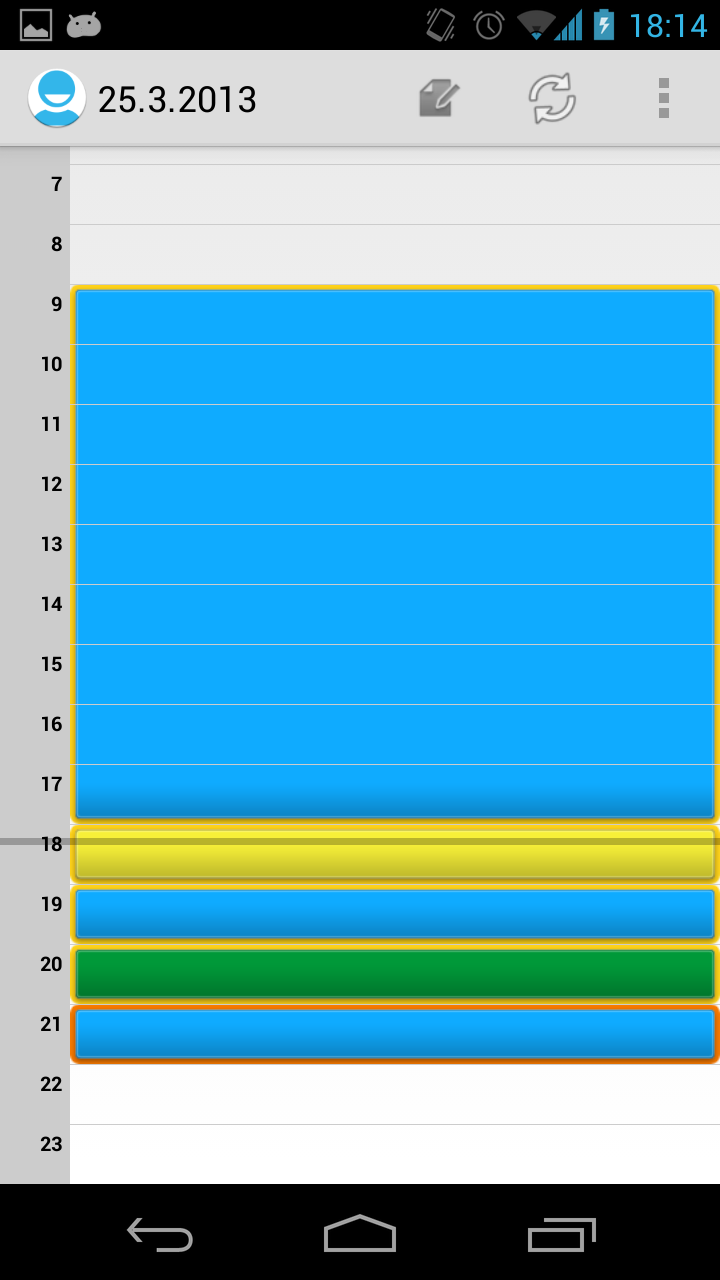
\includegraphics[scale=0.3]{scr/time_doch.png}
  \label{}
\end{figure}

\begin{figure}[H]
  \centering
  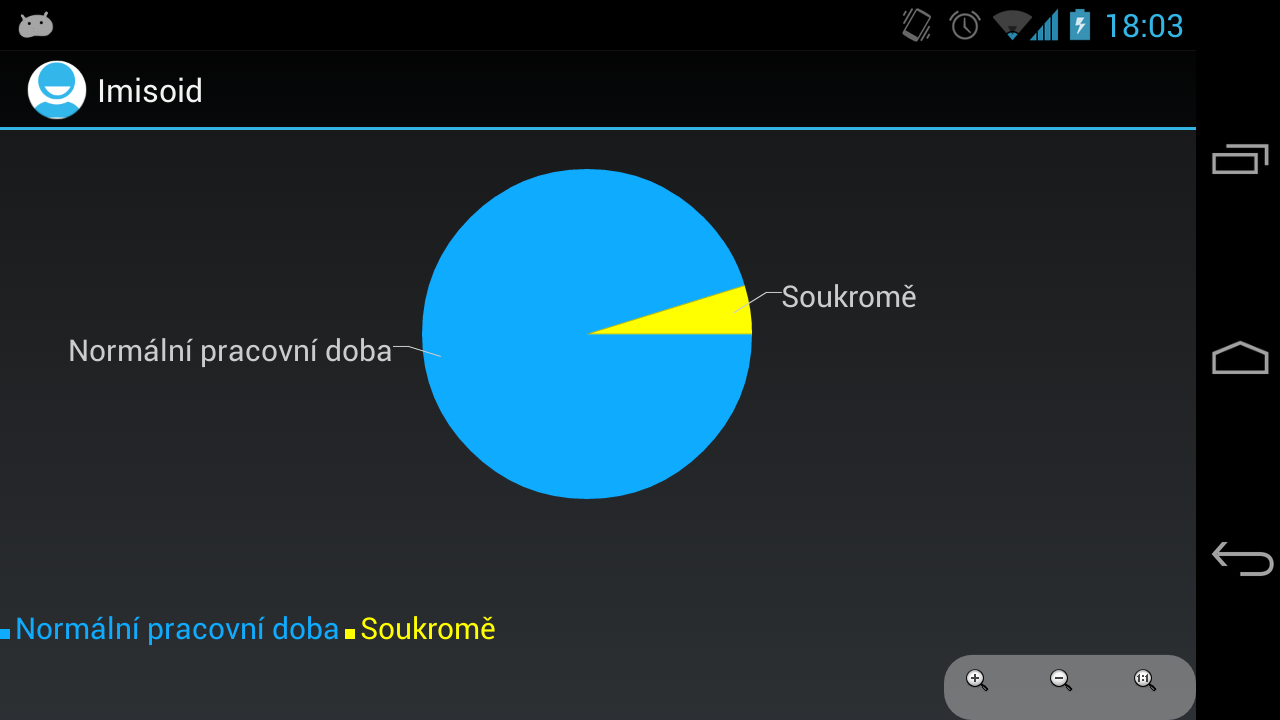
\includegraphics[scale=0.3]{scr/graf_doch.png}
  \label{}
\end{figure}

\begin{figure}[H]
  \centering
  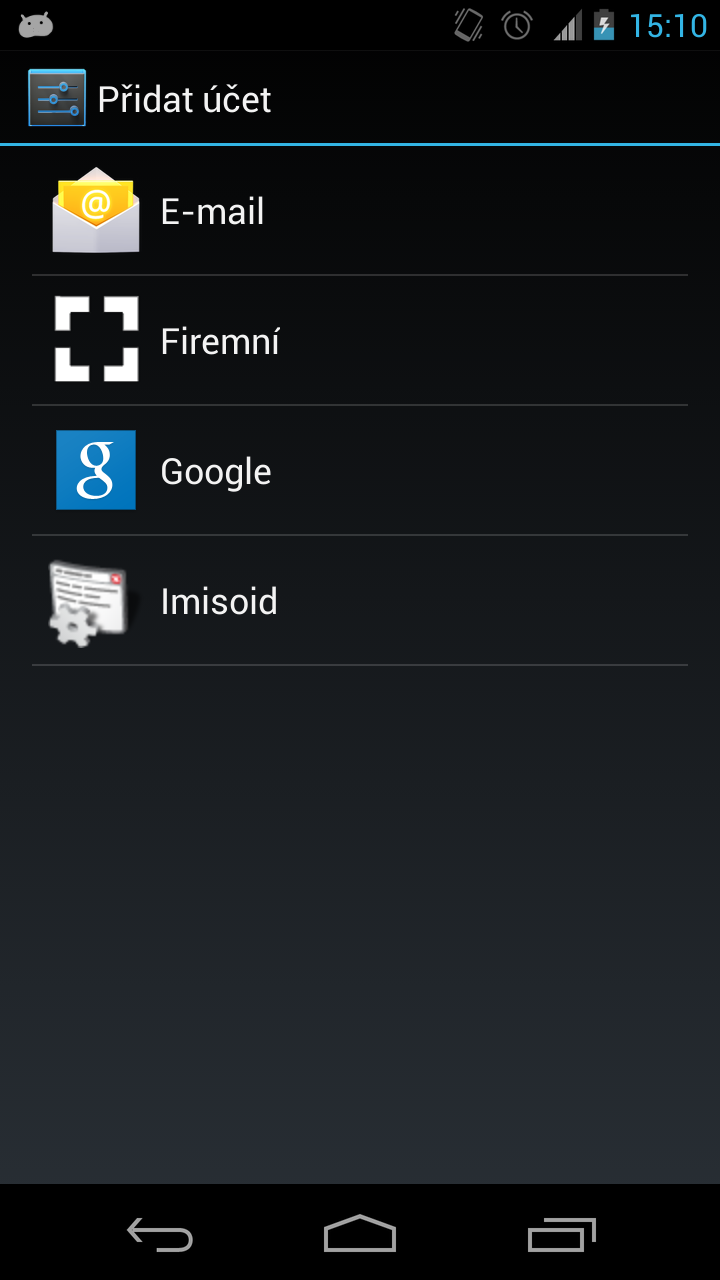
\includegraphics[scale=0.3]{scr/ucet.png}
  \label{}
\end{figure}

\begin{figure}[H]
  \centering
  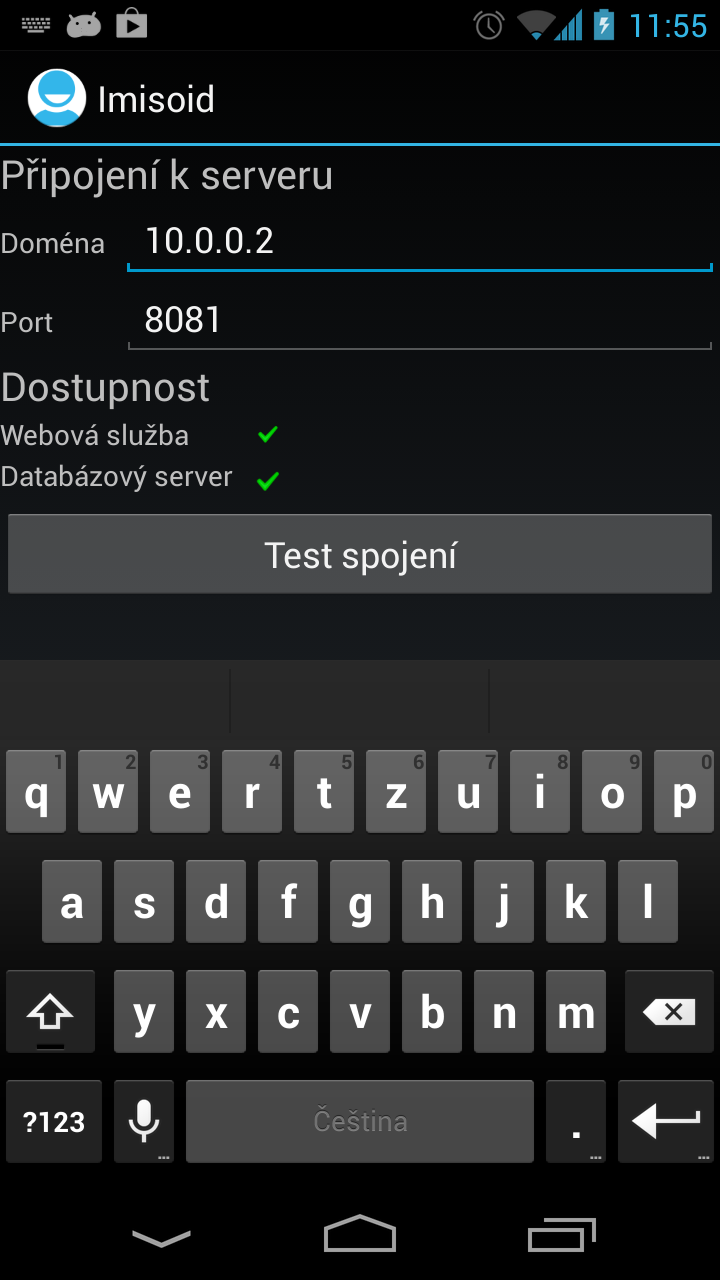
\includegraphics[scale=0.3]{scr/network.png}
  \label{}
\end{figure}
\end{document}
